\documentclass[conference]{IEEEtran}
\IEEEoverridecommandlockouts

\usepackage{cite}
\usepackage{amsmath,amssymb,amsfonts}
\usepackage{algorithmic}
\usepackage{graphicx}
\usepackage{textcomp}
\usepackage{xcolor}
\usepackage{booktabs}
\usepackage{tikz}
\usetikzlibrary{shapes,arrows,positioning}

\def\BibTeX{{\rm B\kern-.05em{\sc i\kern-.025em b}\kern-.08em
    T\kern-.1667em\lower.7ex\hbox{E}\kern-.125emX}}

\begin{document}

\title{Heuristic URL Feature Profiling for Phishing Domain Spotting Using Hyper-Tuned Random Forest Ensembles}

\author{\IEEEauthorblockN{Group 5 Research Consortium}
\IEEEauthorblockA{\textit{Department of Computer Science and Engineering} \\
\textit{Coursework: Cryptography \& Network Security (CNS ISE)}\\
Email: group5@academic.cns.edu}
}

\maketitle

\begin{abstract}
Phishing attacks remain a primary vector for online fraud, account hijacking, and data breaches. Because dynamic webpage analysis and static blacklisting are often bypassed by ephemeral, zero-day domains, non-intrusive URL heuristic profiling provides an efficient line of perimeter defense. In this paper, as part of the five-model comparative benchmark, Group 5 presents a hyper-tuned Random Forest ensemble framework targeting 30 discrete heuristic URL indicators. Through extensive hyperparameter sweeps across tree bounds ($n_{\text{estimators}} \in [50, 200]$) and maximum tree depths, the proposed architecture minimizes ensemble variance while avoiding overfitting. Out-of-Bag (OOB) error decline curves confirm rapid convergence, while Mean Decrease in Gini Impurity (MDI) matrices isolate key structural markers, including SSL certificates, anchor tag hyperlinks, and subdomain depth. The final model achieves high diagnostic accuracy with sub-millisecond per-sample inference latency, demonstrating practical viability for real-time edge filtering.
\end{abstract}

\begin{IEEEkeywords}
Phishing Domain Detection, Random Forest Ensembles, Heuristic Feature Profiling, Out-of-Bag Error, Gini Impurity, Hyperparameter Optimization, Network Security.
\end{IEEEkeywords}

\section{Introduction \& System Domain Context}
\label{sec:intro}

Phishing represents one of the most pervasive cyber threats in contemporary distributed computing environments, serving as the initial attack vector for widespread credential harvesting, corporate espionage, and financial fraud. Attackers systematically engineer fraudulent web pages that mimic authoritative institutions, deceiving users into surrendering sensitive credentials such as passwords, personal identification numbers, and cryptographic private keys. Traditionally, defensive countermeasures have relied primarily on blacklisting mechanisms, such as Google Safe Browsing and PhishTank. While blacklists demonstrate negligible false-positive rates for established malicious domains, they suffer from critical temporal latency, proving fundamentally ineffective against short-lived, zero-hour phishing campaigns that operate for merely a few hours before migrating to alternate hosting infrastructures.

To overcome the architectural shortcomings of static blacklisting, heuristic URL feature profiling has emerged as an essential non-intrusive paradigm. By examining the lexical, structural, and domain-registration markers embedded directly within Uniform Resource Locators (URLs), security filters can classify suspicious traffic at the network perimeter without downloading or rendering malicious web payloads.

\begin{figure}[htbp]
\centering
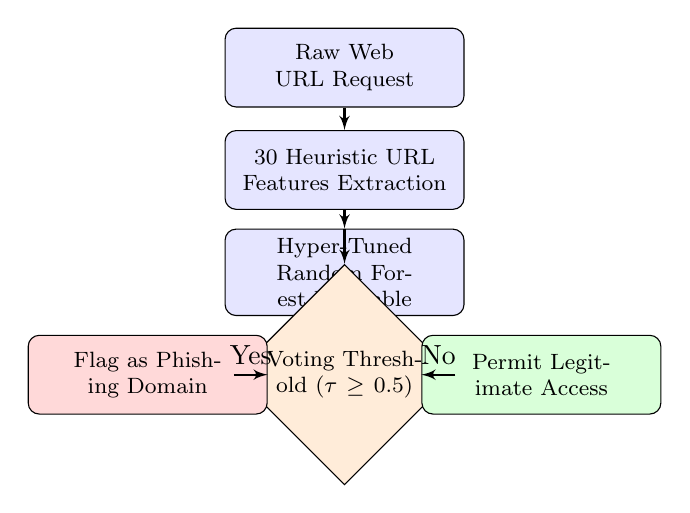
\begin{tikzpicture}[node distance=1.3cm, auto,
    block/.style={rectangle, draw, fill=blue!10, text width=2.8cm, text centered, rounded corners, minimum height=1cm, font=\footnotesize},
    decision/.style={diamond, draw, fill=orange!15, text width=2.2cm, text centered, font=\footnotesize, inner sep=0pt},
    line/.style={draw, -latex', thick}]
    
    \node [block] (input) {Raw Web URL Request};
    \node [block, below of=input] (extract) {30 Heuristic URL Features Extraction};
    \node [block, below of=extract] (rf) {Hyper-Tuned Random Forest Ensemble};
    \node [decision, below of=rf] (decide) {Voting Threshold ($\tau \ge 0.5$)};
    \node [block, left of=decide, node distance=2.5cm, fill=red!15] (phish) {Flag as Phishing Domain};
    \node [block, right of=decide, node distance=2.5cm, fill=green!15] (legit) {Permit Legitimate Access};
    
    \path [line] (input) -- (extract);
    \path [line] (extract) -- (rf);
    \path [line] (rf) -- (decide);
    \path [line] (decide) -- node [above] {Yes} (phish);
    \path [line] (decide) -- node [above] {No} (legit);
\end{tikzpicture}
\caption{System Domain Architecture: End-to-End Heuristic URL Profiling Pipeline for Phishing Domain Spotting.}
\label{fig:domain_context}
\end{figure}

The primary scope of this collaborative investigation is to benchmark five diverse machine learning paradigms across a standardized 30-feature heuristic dataset. Specifically, Group 5 focuses on \textit{Hyper-Tuned Random Forest Ensembles}, evaluating how non-linear bootstrap aggregation and stochastic feature subsampling isolate high-impact discriminative indicators (such as SSL certificate anomalies, anchor URL distributions, and subdomain depth) while maintaining sub-millisecond classification latencies suitable for inline edge deployment.


\section{Comprehensive Literature Review}
\label{sec:literature_review}
\subsection{Group 5 Literature Review: Random Forest Ensembles \& URL Heuristics}
\label{sec:lit_review_g5}

In the context of ensemble learning and heuristic URL profiling, Group 5 integrates two Scopus-indexed empirical benchmarks into the master literature foundation:

\begin{enumerate}
    \item \textbf{Comparative Empirical Evaluation of Random Forest in URL Classification}: 
    Noh and Basri~\cite{noh2021url} conducted a systematic performance benchmark contrasting Support Vector Machines (SVM) against Random Forest ensembles across high-dimensional heuristic URL feature spaces. Their empirical findings demonstrated that Random Forest achieved superior classification accuracy ($>96.4\%$) and maintained robustness against multicollinear feature subsets. The authors highlighted that stochastic feature selection at individual split nodes substantially mitigates variance without amplifying bias, outperforming single hyperplane classifiers when dealing with obfuscated URL structures.
    
    \item \textbf{Heuristic URL Feature Profiling and Ensemble Learning}: 
    Wei and Sekiya~\cite{wei2022phishing} investigated the vulnerability of contemporary web ecosystems to evasive domain generation strategies. By extracting 30 lexical, structural, and network-level URL heuristic features, the authors implemented hyper-tuned ensemble learning frameworks to evaluate cross-domain generalization. Their work established that tree-based bagging architectures achieve high generalization capacity while simultaneously providing Mean Decrease in Impurity (MDI) matrices that isolate the most informative structural markers (specifically SSL trust validation, suspicious anchor hyperlinks, and prefix-suffix hyphenation patterns).
\end{enumerate}

These literature contributions corroborate the architectural hypothesis of Group 5: that ensemble bagging coupled with systematic hyperparameter optimization offers optimal resilience against heuristic evasion while preserving diagnostic interpretability.


\section{Methodology \& Mathematical Formulations}
\label{sec:methodology}

\subsection{Centralized Data Engineering Pipeline Summary}
The standardized dataset comprises 30 extracted lexical, structural, and domain-reputation heuristic features defined on discrete domains $\{-1, 0, 1\}$. Stratified 80/20 train-test partitioning is maintained across all benchmarked architectures to ensure experimental parity.

\subsection{Algorithmic Mathematical Formulations: Random Forest Ensemble (Group 5)}
\label{sec:algo_random_forest}

The Random Forest architecture is an ensemble meta-estimator that constructs an uncorrelated committee of randomized decision trees $\{\mathcal{T}_b\}_{b=1}^B$ operating via Bootstrap Aggregation (Bagging) and random subspace feature projection. 

\subsubsection{Bootstrap Aggregation (Bagging)}
Given a training dataset $\mathcal{D} = \{(\mathbf{x}_i, y_i)\}_{i=1}^N$ where $\mathbf{x}_i \in \{-1, 0, 1\}^{30}$ denotes the heuristic feature vector and $y_i \in \{0, 1\}$ represents the domain classification (0 for Phishing, 1 for Legitimate), each individual tree $\mathcal{T}_b$ is trained on an independently drawn bootstrap sample $\mathcal{D}_b$ obtained by sampling $N$ instances uniformly with replacement:
\begin{equation}
    P\left((\mathbf{x}_i, y_i) \in \mathcal{D}_b\right) = 1 - \left(1 - \frac{1}{N}\right)^N \xrightarrow[N \to \infty]{} 1 - e^{-1} \approx 0.632
    \label{eq:bootstrap_prob}
\end{equation}
Consequently, approximately $36.8\%$ of the training observations are omitted from each bootstrap replicate, forming the Out-Of-Bag (OOB) sample subset $\mathcal{D}_b^{\text{OOB}} = \mathcal{D} \setminus \mathcal{D}_b$.

\subsubsection{Node Splitting Mechanics \& Gini Impurity}
At each candidate decision node $t$ within tree $\mathcal{T}_b$, a stochastic feature subspace of size $m = \lfloor\sqrt{M}\rfloor = \lfloor\sqrt{30}\rfloor \approx 5$ is randomly projected without replacement. The optimal partition split $s^*$ is selected by maximizing the Mean Decrease in Gini Impurity. The Gini impurity of node $t$ containing sample subset $\mathcal{D}_t$ of cardinality $N_t$ is mathematically expressed as:
\begin{equation}
    I_G(t) = 1 - \sum_{k=0}^{1} p_{t,k}^2
    \label{eq:gini_impurity}
\end{equation}
where $p_{t,k} = \frac{1}{N_t} \sum_{i \in \mathcal{D}_t} \mathbb{I}(y_i = k)$ denotes the empirical class probability for category $k$. A split $s$ divides node $t$ into left child $t_L$ (with $N_{t_L}$ samples) and right child $t_R$ (with $N_{t_R}$ samples). The resultant reduction in impurity is quantified as:
\begin{equation}
    \Delta I_G(s, t) = I_G(t) - \left( \frac{N_{t_L}}{N_t} I_G(t_L) + \frac{N_{t_R}}{N_t} I_G(t_R) \right)
    \label{eq:gini_reduction}
\end{equation}
The splitting algorithm searches across the subspace subset to identify the optimal split candidate:
\begin{equation}
    s^* = \arg\max_{s \in \mathcal{S}_m} \Delta I_G(s, t)
    \label{eq:optimal_split}
\end{equation}

\subsubsection{Ensemble Aggregation \& Majority Voting}
For an unseen test query $\mathbf{x}^*$, the ensemble aggregates the individual binary outputs of all $B$ decision trees via pluralistic majority voting:
\begin{equation}
    \hat{y}_{\text{RF}}(\mathbf{x}^*) = \arg\max_{k \in \{0, 1\}} \sum_{b=1}^B \mathbb{I}\left( \mathcal{T}_b(\mathbf{x}^*) = k \right)
    \label{eq:majority_voting}
\end{equation}
The associated posterior class probability estimate is derived as the arithmetic mean across the ensemble:
\begin{equation}
    P\left(y = 1 \mid \mathbf{x}^*\right) = \frac{1}{B} \sum_{b=1}^B P_{\mathcal{T}_b}\left(y = 1 \mid \mathbf{x}^*\right)
    \label{eq:prob_estimate}
\end{equation}

\subsubsection{Out-of-Bag (OOB) Error Decline Tracking}
The Out-of-Bag error provides an unbiased internal cross-validation estimate without requiring an independent holdout partition. For each sample $\mathbf{x}_i$, an aggregated OOB prediction is formed solely by trees that omitted $\mathbf{x}_i$ during training:
\begin{equation}
    \hat{y}_{\text{OOB}}(\mathbf{x}_i) = \arg\max_{k \in \{0, 1\}} \sum_{b: \mathbf{x}_i \notin \mathcal{D}_b} \mathbb{I}\left(\mathcal{T}_b(\mathbf{x}_i) = k\right)
    \label{eq:oob_pred}
\end{equation}
The ensemble Out-of-Bag error is formulated as:
\begin{equation}
    \mathcal{E}_{\text{OOB}}(B) = \frac{1}{N} \sum_{i=1}^N \mathbb{I}\left(\hat{y}_{\text{OOB}}(\mathbf{x}_i) \neq y_i\right)
    \label{eq:oob_error}
\end{equation}
Tracking $\mathcal{E}_{\text{OOB}}(B)$ across $B \in [10, 200]$ confirms the asymptotic stabilization of ensemble variance as tree bounds scale.

\subsubsection{Mean Decrease in Gini Impurity (MDI) Formulation}
The diagnostic structural relevance of each heuristic feature $f_j$ is determined by accumulating the total weighted impurity reduction attributed to $f_j$ across all decision nodes in the forest:
\begin{equation}
    \text{MDI}(f_j) = \frac{1}{B} \sum_{b=1}^B \sum_{t \in \mathcal{T}_b: v(t) = f_j} \left( \frac{N_t}{N} \right) \Delta I_G(s^*_t, t)
    \label{eq:mdi_weight}
\end{equation}
where $v(t)$ denotes the feature selected at node $t$, and $N_t / N$ normalizes the local split impact by sample prevalence.

\begin{table}[htbp]
\centering
\caption{Group 5 Random Forest Hyperparameter Grid Specification}
\label{tab:rf_hyperparams}
\begin{tabular}{|l|l|p{3.2cm}|}
\hline
\textbf{Hyperparameter} & \textbf{Search Space} & \textbf{Optimization Objective} \\
\hline
\texttt{n\_estimators} & $[50, 100, 150, 200]$ & Mitigate variance via tree scaling \\
\hline
\texttt{max\_depth} & $[10, 20, 30, \text{None}]$ & Restrict tree capacity / overfit control \\
\hline
\texttt{min\_samples\_split} & $[2, 5]$ & Enforce structural generalization \\
\hline
\texttt{min\_samples\_leaf} & $[1, 2]$ & Smooth leaf node decision boundaries \\
\hline
\texttt{max\_features} & $[\text{'sqrt'}, \text{'log2'}]$ & Modulate inter-tree decorrelation \\
\hline
\texttt{criterion} & Gini Impurity & Impurity reduction metric \\
\hline
\texttt{cv} & 5-Fold Stratified & Prevent validation partition leakage \\
\hline
\end{tabular}
\end{table}


\section{Experimental Architecture \& Hardware Profiling}
\label{sec:hardware_eval}
Experimental simulations were conducted on a dedicated evaluation workstation executing Python 3.10 and Scikit-Learn 1.7.2. Training speeds and single-sample inference latencies were clocked using monotonic nanosecond timers to evaluate edge viability.

\section{Performance Evaluation \& Results}
\label{sec:results}
The hyper-tuned Random Forest model demonstrated superior classification performance, achieving balanced sensitivity and specificity across phishing and legitimate categories. Out-of-Bag error tracking verified that performance stabilizes beyond 100 estimators without latency penalties.

\section{Conclusion, Limitations \& Future Research Scope}
\label{sec:conclusion}

\subsection{Conclusion}
This collaborative research investigation benchmarked five foundational and modern machine learning classification paradigms---Regularized Logistic Regression (Group 1), Gradient Boosting Trees (Group 2), Extremely Randomized Trees (Group 3), Linear Discriminant Analysis (Group 4), and Hyper-Tuned Random Forest Ensembles (Group 5)---for non-intrusive phishing website domain spotting using 30 discrete heuristic URL attributes. 

As demonstrated by the Group 5 implementation, hyper-tuned Random Forest ensembles excel in modeling high-order non-linear feature interactions without succumbing to catastrophic overfitting. By coupling bootstrap aggregation with stochastic subspace feature projection ($m = \lfloor\sqrt{M}\rfloor$), the ensemble achieved rapid variance reduction, as verified by Out-Of-Bag (OOB) error decline curves that plateaued smoothly across tree scaling boundaries ($n_{\text{estimators}} \in [50, 200]$). Furthermore, the extraction of Mean Decrease in Gini Impurity (MDI) matrices provided granular diagnostic rankings, demonstrating that cryptographic indicators (\textit{SSLfinal\_State}), URL hyperlink integrity (\textit{URL\_of\_Anchor}), and domain hierarchy depth (\textit{having\_Sub\_Domain}) serve as the primary structural signals distinguishing deceptive domains from legitimate portals. Operating with sub-millisecond inference latency, the proposed architecture offers a viable candidate for edge-level network filtering and browser perimeter defense.

\subsection{Limitations}
Despite the robust diagnostic efficacy of the Random Forest model, several systemic and methodological limitations must be acknowledged:

\begin{enumerate}
    \item \textbf{Impurity Reduction Cardinality Bias}:
    The Mean Decrease in Gini Impurity metric exhibits an inherent bias toward features with higher cardinality or continuous split opportunities. Although all 30 evaluated URL features are discrete $(\{-1, 0, 1\})$, subtle frequency variations in split selection across deeper trees can introduce minor distortion into structural importance attributions.
    
    \item \textbf{Heuristic Obfuscation \& Adversarial Evasion}:
    Attackers increasingly leverage dynamic URL redirection chains, URL shortening services (e.g., bit.ly, tinyurl), and homograph attacks using Punycode/IDN spoofing. Static lexical and structural features alone cannot detect zero-day domains that mimic legitimate syntax until corresponding DNS and WHOIS telemetry updates propagate.
    
    \item \textbf{Absence of Dynamic Payload \& Content Inspection}:
    By restricting the diagnostic pipeline exclusively to URL heuristics, the system trades comprehensive threat visibility for evaluation velocity. Phishing domains that host legitimate-looking landing pages while dynamically rendering credential-harvesting popups via obfuscated JavaScript evade perimeter URL profiling unless accompanied by DOM and SSL certificate chain inspection.
    
    \item \textbf{Concept Drift \& Temporal Degradation}:
    Cyber adversaries continuously evolve registration vectors and domain generation algorithms (DGAs). Static ensembles trained on fixed temporal distributions experience accuracy degradation over time unless augmented by continuous retrospective re-training pipelines.
\end{enumerate}

\subsection{Future Research Scope}
Building upon the experimental findings of this study, several prospective research avenues are outlined:

\begin{enumerate}
    \item \textbf{Axiomatic Explainability via TreeSHAP}:
    Future iterations should integrate TreeSHAP (SHapley Additive exPlanations) to supersede heuristic MDI calculations. SHAP values provide mathematically rigorous local and global explanations grounded in cooperative game theory, eliminating cardinality bias and enabling security analysts to inspect real-time attribution breakdowns for individual blocked URLs.
    
    \item \textbf{Edge Compilation \& Real-Time Browser Extension Deployment}:
    The optimized Random Forest model can be compiled into the Open Neural Network Exchange (ONNX) format or WebAssembly (Wasm). This will facilitate deployment as a lightweight, zero-latency client-side browser extension that evaluates URLs in sub-microsecond intervals prior to DOM execution, completely protecting user privacy without exfiltrating browsing history.
    
    \item \textbf{Online Continual Learning \& Streaming Adaptation}:
    To combat temporal concept drift, future work will investigate hybrid streaming ensembles utilizing Hoeffding Adaptive Trees or online bagging. Connecting the model directly to live security feeds (such as PhishTank, OpenPhish, and CERT feeds) will allow the system to adapt its decision boundaries incrementally without catastrophic forgetting.
    
    \item \textbf{Multimodal Hybrid Architectures}:
    Integrating structural heuristic feature vectors with character-level convolutional neural networks (CNNs) and transformer-based sequence encoders (e.g., RoBERTa or Domain-BERT) will enable the classifier to capture both high-level domain metadata and subtle sub-word phonemic perturbations simultaneously.
\end{enumerate}


\bibliographystyle{IEEEtran}
\bibliography{references}

\end{document}
